
\chapter{Running CFAST}

Running CFAST is relatively simple. All of the parameters that describe a given fire scenario are entered into a text file that is referred to as the "data" or "input" file. In this document, the data file is designated as filename.in, where "filename" stands for any character string that helps to identify the simulation. All of the output files associated with the calculation would typically have this common prefix. In addition to the input file, there are often several external files containing input parameters for the simulation. These files are referred to as "database" files, which contain parameters describing common materials and fuels.

The CFAST distribution includes a Windows-based input editor called CEdit that allows the user to enter details of a simulation in a standard Windows format, save the data file to disk, and run the simulation with CFAST from within the program.  Typically, all simulations would be developed and run from within CEdit.  For numerous, similar or lengthy simulations, the fire model CFAST can be run from a command prompt window.

It is suggested that a new user start with an existing data file, run it as is, and then make the appropriate changes to the input file for the desired scenario. By running a sample case, the user becomes familiar with the procedure and ensures that his/her computer is up to the task before embarking on learning how to create new input files.

\section{Creating a CFAST Input Data File}

All of the data to run the model is contained in an input data file. This file contains information about the building geometry (compartment sizes, materials of construction, and material properties), connections between compartments (horizontal flow openings such as doors, windows), vertical flow openings in floors and ceilings, and mechanical ventilation connections), fire properties (fire size and species production rates as a function of time), and specifications for detectors, sprinklers, and targets (position, size, heat transfer characteristics, and flow characteristics for sprinklers). Materials are defined by their thermal conductivity, specific heat, density, thickness, and burning behavior (heat release rate, ignition properties, and species yields).

The input data file provides the program with parameters to describe the scenario under consideration. The parameters are organized into groups of related variables. Each line of the input data file contains inputs related to a single group and begins with a keyword that identifies the input.  For example, compartment geometry is described by a set of lines (keyword COMPA) that define the width, depth, and height of each compartment.  A description of the input parameters can be found in Chapter 4.

Typically, the input data file will be created with the input editor, CEdit, included with the CFAST distribution. A shortcut to the input editor is placed on the start menu during installation.  To run, select Start, Program Files, and CFAST. Details of the program and its inputs are described in chapter 4.

\begin{figure}[h!]
\begin{center}
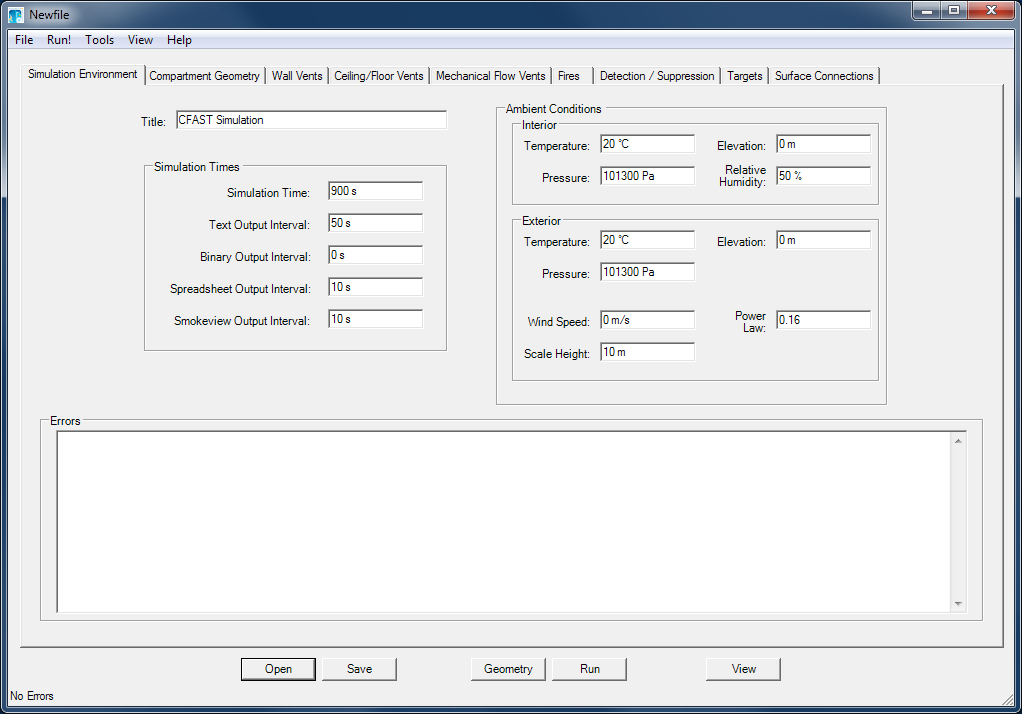
\includegraphics[width=6.5in]{FIGURES/Running_CFAST/Environment_Tab}
\end{center}
\end{figure}

\begin{wrapfigure}{l}{3in}
  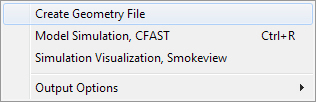
\includegraphics[width=3in]{FIGURES/Running_CFAST/Run_Menu}
\end{wrapfigure}

The program includes a number of menu items for ancillary functions.  In addition to the normal file menu items to open and save input data files or to exit the program, a 'Run!' menu is included to execute or view the current simulation. Menu items include the following:

\textbf{Create Geometry File:} used to create a geometry file for visualization with the program smokeview.  The input data file is saved, if necessary, and CFAST is run with an option to only run through initialization. This is particularly useful to review placement of compartments, vents, and fires in a CFAST scenario. The resulting geometry can be viewed with the 'Simulation Visualization, Smokeview' menu item, below.

\textbf{Model Simulation, CFAST:} runs the current input data file specification with the fire model CFAST.  The input data file is saved, if necessary, and CFAST is run to completion.  Additional details are described below in the section on starting a CFAST calculation. In order to visualize the results of the simulation with the program smokeview, the Smokeview Output Interval must be set to a non-zero value on the simulation Environment page.  This is described in more detail in chapter 4.

\textbf{Simulation Visualization, Smokeview:} runs the program smokeview with the previously defined smokeview geometry file. This allows the user to see the compartment geometry and connections or view the results of the simulation visually.  Additional details on the use of smokeview are included in the user's guide for Smokeview \cite{Smokeview_Users_Guide_6}.

\begin{figure}[h!]
\begin{center}
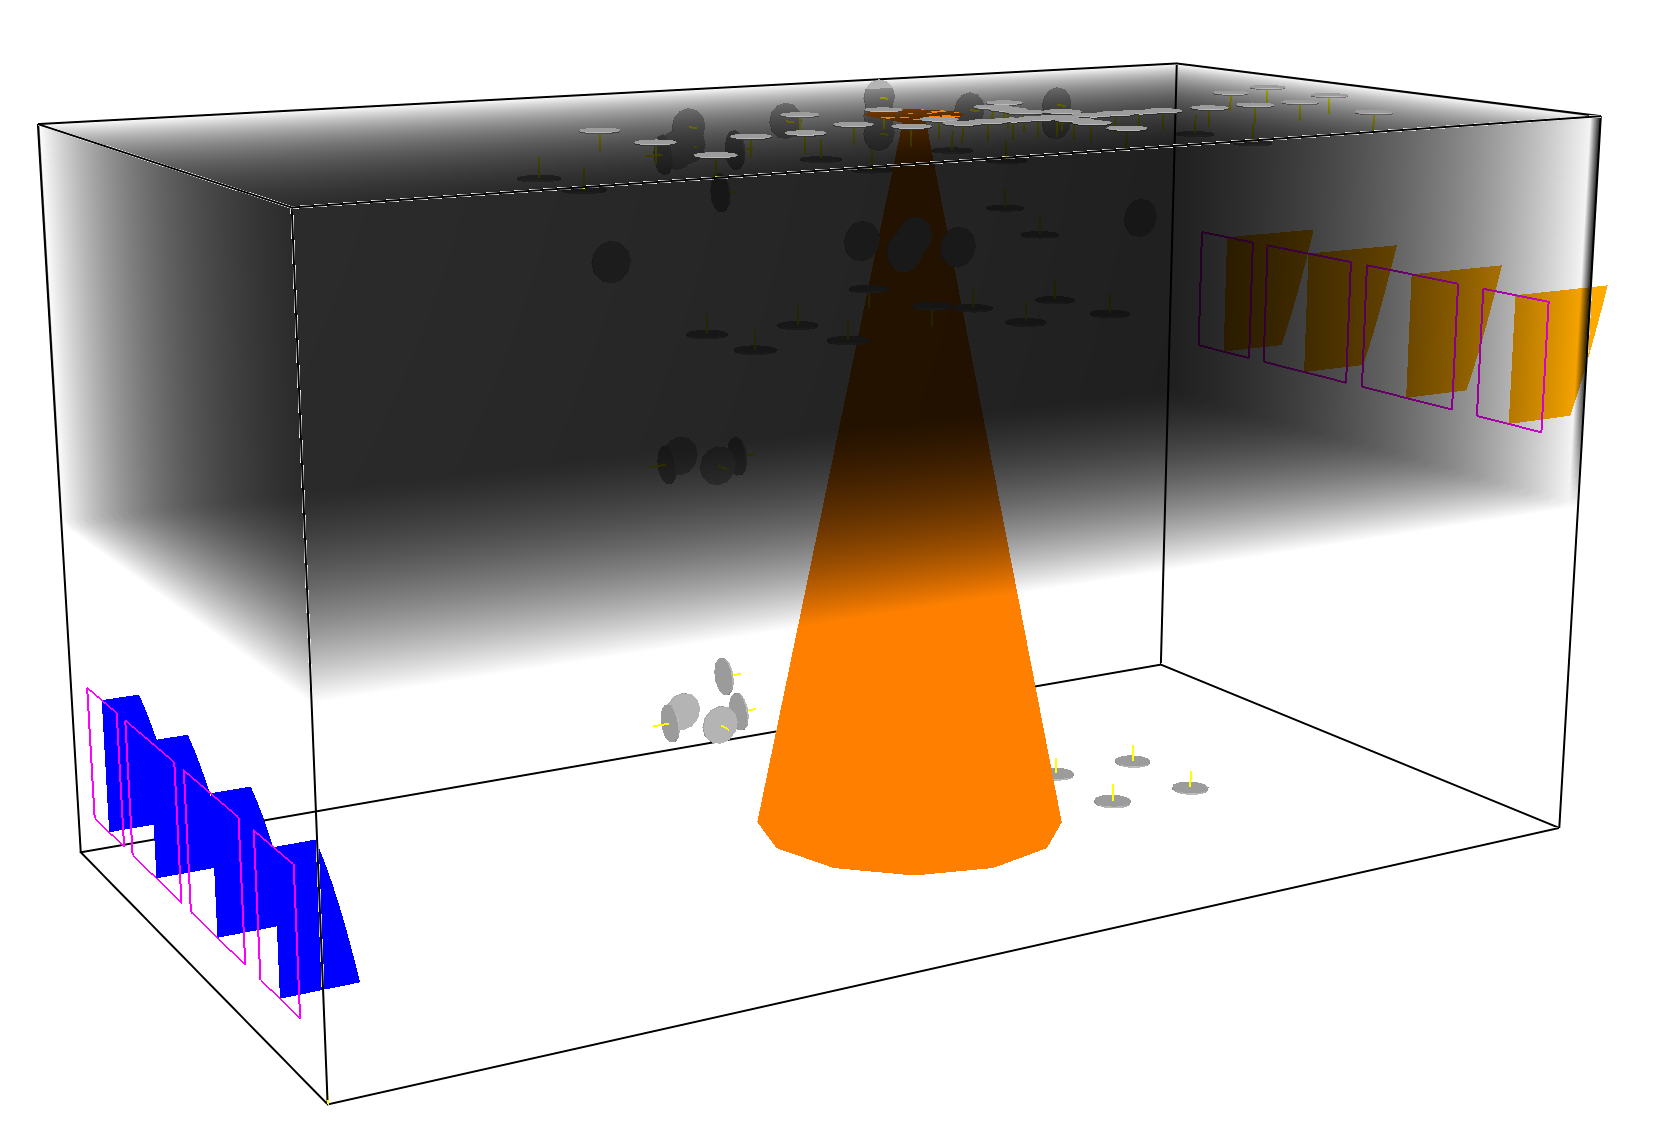
\includegraphics[width=6.5in]{FIGURES/Running_CFAST/Smokeview_Sample}
\end{center}
\end{figure}

\newpage

\begin{wrapfigure}{l}{2.6in}
  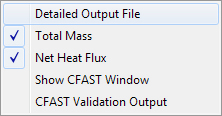
\includegraphics[width=2.6in]{FIGURES/Running_CFAST/Output_Options_Menu}
\end{wrapfigure}

Additional menu items can be selected to control details of the model simulation output using CFAST by selecting the Output Options submenu.

\textbf{Detailed Output File:} If checked, this menu item directs the CFAST model to produce a detailed text output file.  Details of the output are included in chapter 5.

\textbf{Total Mass Output File:} If checked, this menu item directs the CFAST model to replace the flow output with total mass flow through (mechanical) vents rather than the default flow rate values.

\textbf{Net Heat Flux:}  If checked, this menu item directs the CFAST model to calculate heat flux to targets as a net heat flux to the target with the target at ambient temperature rather than at the calculated temperature.  This output is particularly useful to compare predictions to heat flux measurement using water cooled heat flux gauges.

\textbf{Show CFAST Window:} If checked, this menu item allows the user to see the windows command prompt that is used to execute the CFAST model when the Model Simulation, CFAST menu item is used.  By default, this is not checked.  Normally, this can be left unchecked.  For troubleshooting, this can be selected to see additional details of the calculation as it progresses.

\textbf{CFAST Validation Output:} If checked, this menu item directs the CFAST model to output target fluxes at net heat flux and to output an abbreviated heading for spreadsheet columns that are better for automated processing of the data.


\begin{wrapfigure}{l}{2in}
  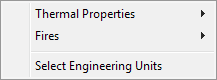
\includegraphics[width=2in]{FIGURES/Running_CFAST/Tools_Menu}
\end{wrapfigure}

The 'Edit' menu allows the user to view or change the material thermophysical properties and fire definitions used by the model and to select desired engineering units used in the input editor CEdit. Menu items include the following.

\textbf{Thermal Properties:} Heat transfer through compartment surfaces, to secondary fire objects, or other targets that may be specified depends on user-specified thermal properties for the materials.  These may be viewed, changed, or added to by the user as desired with the \textbf{Edit Thermal Properties} menu item. Materials properties include thermal conductivity, specific heat, density, thickness, and emissivity. Materials included in the database provided with the program are textbook values of common building and furnishing materials.

\begin{figure}[h!]
\begin{center}
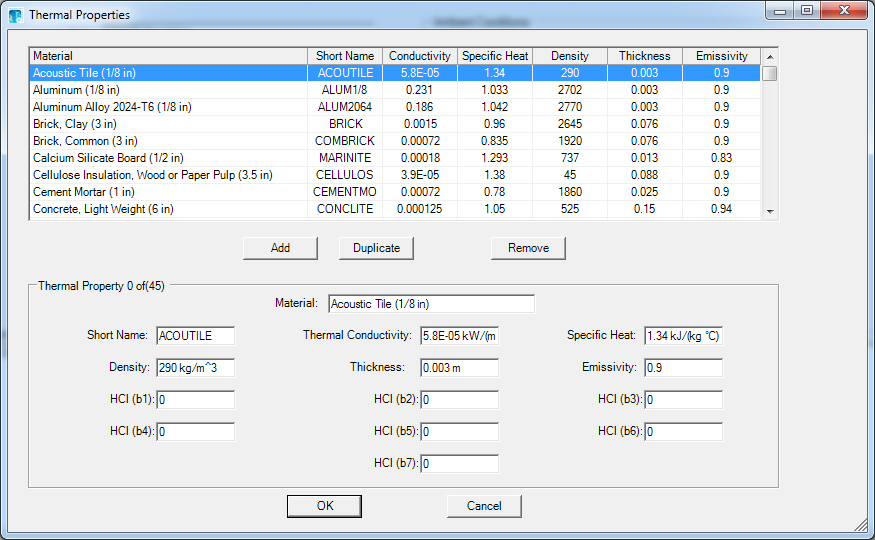
\includegraphics[width=6.5in]{FIGURES/Running_CFAST/Thermal_Properties_Edit}
Editing Thermal Properties in Cedit
\end{center}
\end{figure}

When CEdit is started, no thermal properties or fires are defined.  The \textbf{Insert Thermal Properties} menu item allows thermal properties used in a different simulation to be inserted into the data for the current simulation by choosing an existing CFAST input file and selecting one or more of the thermal properties to be included in the current simulation.

\begin{figure}[h!]
\begin{center}
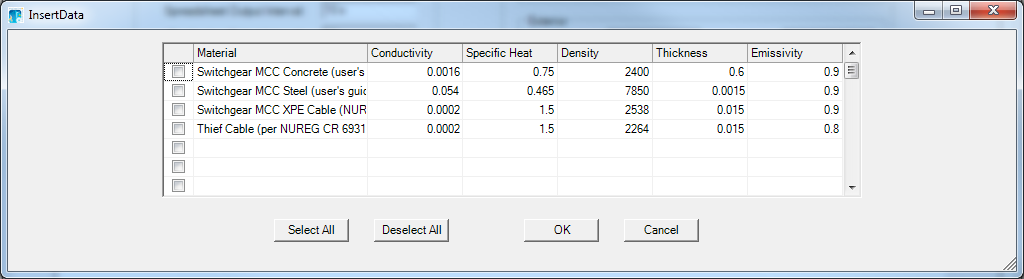
\includegraphics[width=6.5in]{FIGURES/Running_CFAST/Thermal_Properties_Insert}
Inserting Thermal Properties in Cedit
\end{center}
\end{figure}

\newpage

\textbf{Fires:} Fires in CFAST are defined with one or more selected fire objects that define the heat release rate, pyrolysis rate, and species yields as a function of time for each fire.  These may include the default set of fire objects included with the software or additional or modified objects created by the model user. They may be viewed or changed by the user as desired with the \textbf{Edit Fires} menu item.

\begin{figure}[h!]
\begin{center}
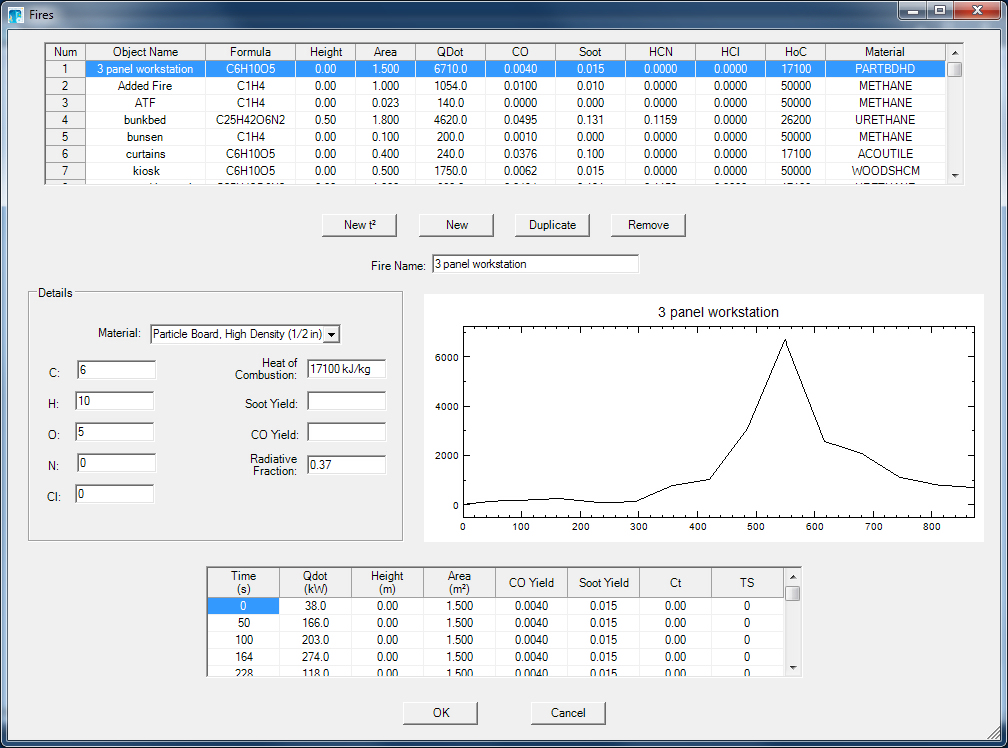
\includegraphics[width=6.5in]{FIGURES/Running_CFAST/Fire_Objects_Edit}
Editing Fires in CFAST
\end{center}
\end{figure}
\newpage

When CEdit is started, no thermal properties or fires are defined.  The \textbf{Insert Fires} menu item allows fire definitions used in a different simulation to be inserted into the data for the current simulation by choosing an existing CFAST input file and selecting one or more of the fires to be included in the current simulation.

\begin{figure}[h!]
\begin{center}
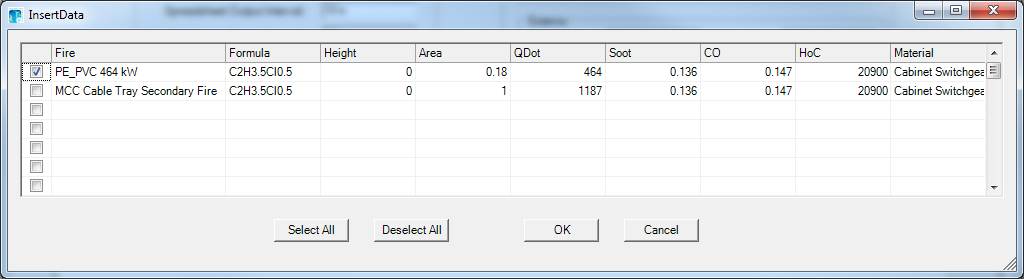
\includegraphics[width=6.5in]{FIGURES/Running_CFAST/Fire_Objects_Insert}
Inserting Fires in Cedit
\end{center}
\end{figure}

Details of fire objects and parameters included on the fire objects window are included in the section on object fires in the next chapter.

\textbf{Select Engineering Units:} The CFAST model uses input values and provides output in S.I. units. Within the input editor, CEdit, the user may select engineering units of choice for input and output.  These values are saved in the windows registry and may be changed at any time. By default, most outputs are in S.I. units, with temperature in Celsius.

\begin{wrapfigure}{l}{3in}
  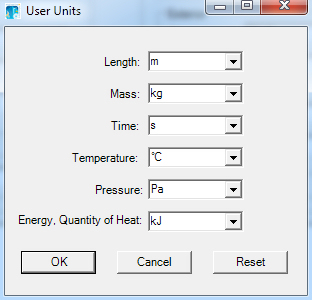
\includegraphics[width=3in]{FIGURES/Running_CFAST/Select_Engineering_Units}
\end{wrapfigure}

\clearpage

\begin{wrapfigure}{r}{1.95in}
  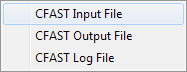
\includegraphics[width=1.95in]{FIGURES/Running_CFAST/View_Menu}
\end{wrapfigure}

The View menu allows the user to view and / or print the input data file, output file (if the simulation has been run and a text output file generated) and the log file of the simulation. If one of the items does not exist on the user's hard disk, the selection is grayed out. \\~ \\

\begin{wrapfigure}{r}{1.88in}
  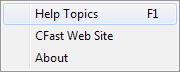
\includegraphics[width=1.88in]{FIGURES/Running_CFAST/Help_Menu}
\end{wrapfigure}
 The Help menu accesses this user's guide, the CFAST web site, or an about dialog box that displays the user license and version of the program. \\~ \\

\section{File Naming and Location}

By default, the CFAST installation places all program files in the directory 'c:$\backslash$Program Files$\backslash$CFAST6' (or directory 'c:$\backslash$Program Files (x86)$\backslash$CFAST6'  on Windows 7 machines) and sample input data files in the 'Examples' folder included in the installation directory, While these locations can be changed during installation, the documentation in this user's guide assumes these locations.

In addition, there are several files that CFAST uses to communicate with its environment.  They include 1) an input data file, required for every simulation, 2) a series of spreadsheet files of important output variables, and binary data files containing calculated values for visualization the simulation.  Documentation of the input data file is included as chapter 4 of this user's guide.

In CFAST, simulations are arranged as projects with all the files associated with a single simulation sharing a common base file name.  For a simulation with a base file name of 'project', the built-in naming conventions would identify the files of the simulation as follows:

\begin{itemize}
\item input: project.in
\item text output file: project.out
\item spreadsheet output files: (Normal output) project\_n.csv, (Species output) project\_s.csv, (Flow output) project\_f.csv, (Wall surface temperatures, targets and sprinklers) project\_w.csv
\item smokeview geometry file: project.smv
\item smokeview plot file: project.zone
\item smokeview slice file(s): project\_\#\#\#\#.sf (where \#\#\#\# is a four digit number automatically assigned by the software)
\item smokeview iso-surface file(s): project\_\#\#\#\#.iso (where \#\#\#\# is a four digit number automatically assigned by the software).
\end{itemize}

There may be additional files associated with a specific simulation.  Any fires defined for the simulation (fire object files are defined with a .o extension) and customized thermal properties may be included in a revised thermal.csv file.  These must be in the same directory as the input file for the model to run.

\section{Starting a CFAST Calculation}

\subsection{Running CFAST from CEdit}

Typically, model simulations are run directly from the input editor, CEdit.  To run the model, either open an existing input data file from the program menus with 'File', 'Open,' or create a new input data file within CEdit.  The model is run by selecting 'Run!' and then 'Model Simulation, CFAST.'

This opens a window that shows the progress of the simulation, with information on the environment in each compartment of the simulation.

\begin{figure}[h!]
\begin{center}
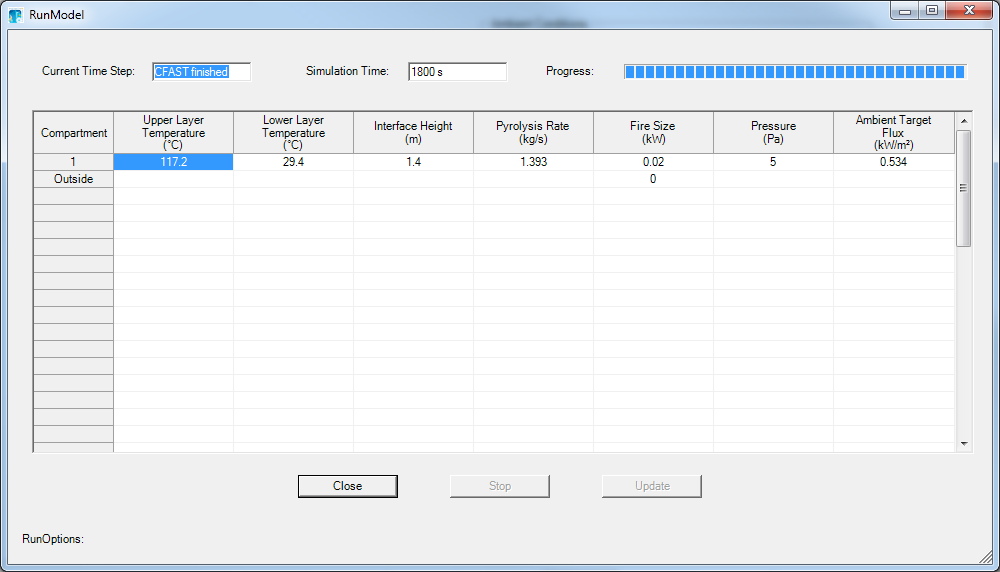
\includegraphics[width=6.5in]{FIGURES/Running_CFAST/Standard_Output}
\end{center}
\end{figure}

Several buttons are also available as follows:

\begin{wrapfigure}{l}{0pt}
  
\includegraphics[width=0.79in]{FIGURES/Running_CFAST/Close_Button}
\end{wrapfigure}

The close button is disabled while the model is running.  Once the simulation is complete (stopped by the user with the stop button), the close button closes the window and returns to the main input editor. \\

\begin{wrapfigure}{l}{0pt}
  
\includegraphics[width=0.79in]{FIGURES/Running_CFAST/Stop_Button}
\end{wrapfigure}

 The stop button halts execution of the simulation, but leaves the simulation window on the screen.  The stop button is available only when the simulation is in progress. \\

Normally, model outputs are displayed and updated only at any of the time intervals specified on the environment page. For complex calculations, there may be a significant time period between display updates. The update button allows the user to see the current state of the calculation at any time. The update button is only available when the simulation is in progress.

\subsection{Running CFAST from a Command Prompt}

The model CFAST can also be run from a Windows command prompt.  CFAST can be run from any folder, and refer to a data file in any other folder. The fires and thermophysical properties have to be in either the data folder, or the executable folder. The data folder is checked first and then the executable folder.

\begin{lstlisting}
[drive1:\][folder1\]cfast [drive2:\][folder2\]project
\end{lstlisting}

The project name will have extensions appended as needed (see below). For example, to run a test case when the cfast executable is located in c:$\backslash$nist$\backslash$cfast6 and the input data file is located in c:$\backslash$data, the following command could be used:

\begin{lstlisting}
c:\nist\cfast6\cfast c:\data\testfire0   <<< note there is no extension.
\end{lstlisting}

If the command is entered as $\backslash$bin$\backslash$cfast $\backslash$bin$\backslash$data$\backslash$testfire0.in, then CFAST will try to open testfire0.in.in

The database files for thermal properties and fire objects may be located either in the folder with the input data file or in the folder with the cfast executable. The model checks first in the data file folder and then in the cfast executable folder.  If the files do not exist in either location, the simulation is not run. By default, names for these files are thermal.csv for the thermal properties file and *.o for the fire object files.

Command line options

\begin{itemize}
\item k - no keyboard access
\item i - initialization only
\item h - output header
\item c - compact output
\item f - full output (c and f are exclusive). Note the interaction of the f and c option. The default for the console output is /c. The default for the file output is /f. This default action can be overwritten by explicitly including the /f or /c option. Output goes to the screen if the print interval (second entry on the TIMES line) is positive and to the output file if the interval is negative.
\item t - replace the flow output with total flow through (mechanical) vents.
\item n - net heat flux option
\item v - validation output (outputs a modified set of spreadsheet files with different column headers designed to facilitate automated analysis of the output)
\end{itemize}
